\documentclass[tikz,border=8pt]{standalone}
% Shared look for every TikZ diagram. Load with \input{../../tools/tikz-style.tex}
\usepackage[T1]{fontenc}
\usepackage{lmodern}
\renewcommand{\sfdefault}{lmr}  % diagrams use the same serif as the text
\usetikzlibrary{arrows.meta, positioning, shapes.geometric, calc, fit, backgrounds}
\definecolor{cblue}{HTML}{4C78A8}
\definecolor{corange}{HTML}{F58518}
\definecolor{cgreen}{HTML}{54A24B}
\definecolor{cred}{HTML}{E45756}
\definecolor{cpurple}{HTML}{B279A2}
\definecolor{cgrey}{HTML}{6B6B6B}
\tikzset{
  every picture/.style={font=\sffamily, line width=1.2pt},
  box/.style={draw=#1, fill=#1!12, rounded corners=4pt, align=center, inner sep=7pt, minimum height=1.1cm},
  box/.default=cgrey,
  arrow/.style={-{Stealth[length=3mm]}, draw=cgrey, line width=1.4pt},
  title/.style={font=\sffamily\bfseries\Large},
  note/.style={font=\sffamily\small, text=cgrey, align=center},
}
\AtBeginDocument{\hyphenpenalty=10000 \exhyphenpenalty=10000}

% A flat as a metric map (rooms drawn to scale) and as a topological map (places as nodes, ways between them as edges).
\begin{document}
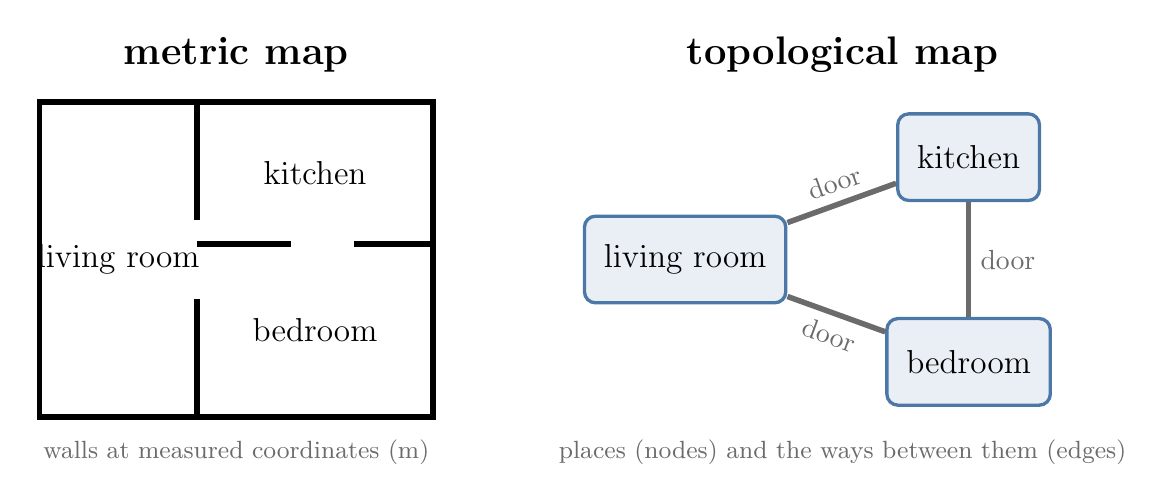
\begin{tikzpicture}[every node/.append style={font=\large}]
  \node[title] at (2.5,4.6) {metric map};
  \draw[black, line width=2pt] (0,0) rectangle (5,4);
  \draw[black, line width=2pt] (2,0) -- (2,1.5); \draw[black, line width=2pt] (2,2.5) -- (2,4);
  \draw[black, line width=2pt] (2,2.2) -- (3.2,2.2); \draw[black, line width=2pt] (4.0,2.2) -- (5,2.2);
  \node at (1,2) {living room}; \node at (3.5,3.1) {kitchen}; \node at (3.5,1.1) {bedroom};
  \node[note] at (2.5,-0.45) {walls at measured coordinates (m)};
  \begin{scope}[xshift=8.2cm]
    \node[title] at (2,4.6) {topological map};
    \node[box=cblue] (l) at (0,2) {living room};
    \node[box=cblue] (k) at (3.6,3.3) {kitchen};
    \node[box=cblue] (b) at (3.6,0.7) {bedroom};
    \draw[line width=2pt, cgrey] (l) -- node[above, sloped, font=\normalsize] {door} (k);
    \draw[line width=2pt, cgrey] (l) -- node[below, sloped, font=\normalsize] {door} (b);
    \draw[line width=2pt, cgrey] (k) -- node[right, font=\normalsize] {door} (b);
    \node[note] at (2,-0.45) {places (nodes) and the ways between them (edges)};
  \end{scope}
\end{tikzpicture}
\end{document}
